\documentclass[../ZF_SWEN1.tex]{subfiles}

\begin{document}

\subsection{Objektorientierung}

\paragraph{Grundidee: } Reale Welt besteht aus Objekten, die untereinander in Beziehungen stehen.

\begin{itemize}
	\item Klasse:
	\begin{itemize}
		\item Daten(Attribute)
		\item Funktionalität(Operationen, Methoden)
	\end{itemize}
	\item Objekte:
	\begin{itemize}
		\item In der Lage Nachrichten (= Methodenaufrufe) zu empfangen
		\item Daten verarbeiten
		\item Nachrichten senden
		\item können einmal erstellt werden
		\item in verschiedene Kontexten wiederverwendet werden
	\end{itemize}
\end{itemize}


\paragraph{Objektorientierte Analyse(OOA): } Objekte-Konzepte-in Domäne zu finden und zu beschreiben. \\
\paragraph{Objektorientierten Design (OOD): } Geeignete Softwareobjekte und ihr Kollaboration zu definieren um Anforderungen zu erfüllen.

\paragraph{Domänenschicht: } Klassen abgeleitet aus dem Domänenmodell (Low-Representational-Gap)


\subsubsection{Use Cases und System-Sequenzdiagramm}
\paragraph{Basis für das Design: }
\begin{enumerate}
	\item Szenarien
	\item Systemoperationen
	\item Domänenmodell
\end{enumerate}

\subparagraph{Was programmiert werden muss: }
\begin{enumerate}
	\item Systemoperationen bzw. deren Antworten
\end{enumerate}


\paragraph{Use-Case-Realisierung: } Wie ein bestimmter Use Case innerhalb Design mit kollaborierenden Objekten realisiert wird.

\paragraph{Systemoperationen: } Jedes Szeanario schrittweise entworfen und implementiert

\paragraph{UML-Diagramme: } Gemeinsame Sprache um Use-Case-Realisierungen zu veranschaulichen und zu diskutieren.


\subsubsection{Klassen entwerfen: }
Zwei arten von Design-Modellen (ergänzen sich und werden parallel erstellt):
\begin{itemize}
	\item Statische Modelle:
	\begin{itemize}
		\item \textcolor {orange}{UML-Klassendiagramm}- Unterstützen Entwurf Paketen, Klassennamen, Atrributen und Methodensignaturen (ohne Methodenkörperd)
	\end{itemize}
	\item Dynamische Modelle:
	\begin{itemize}
		\item \textcolor {orange} {UML-Interaktionsdiagramme} Untersützen Entwurf der Logik, des Verhaltens des Codes und der Methodenkörper.
	\end{itemize}	
\end{itemize}


\subsection{UML-Diagramme für das Design}
\subsubsection{Grundelemente der UML}
\begin{itemize}
	\item Primitiver Datentyp
	\item Literal
	\item Schlüsselwort, Stereotyp
	\item Randbedingung (constraint)
	\item Kommentar
	\item Diagrammrahmen (optional)
\end{itemize}

\begin{figure}[H]
\centering
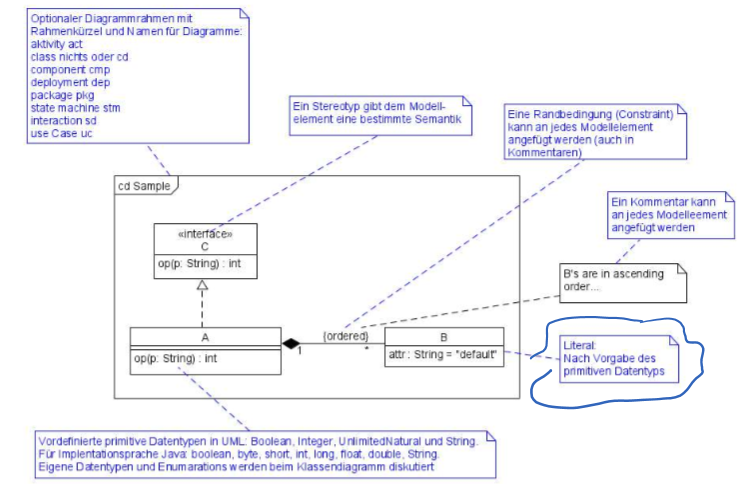
\includegraphics[width=0.3\textwidth]{/Resources/Images/Grundelemente_Klassendiagramm.png}
\caption{\label{fig:Grundelemente_Klassendiagramm}Grundelemente\_Klassendiagramm.}
\end{figure}

\subsection{UML-Klassendiagramm}
\begin{itemize}
	\item Statische struktur
	\item Konzeptuell: Problemdomäne (Domänenmodell)
	\item Design: Lösungsdomäne (DCD)
\end{itemize}

\subsubsection{Notationselemente}
\begin{itemize}
	\item Klasse
	\item Attribut
	\item Operation
	\item Sichtbarkeit von Attributen und Operationen
	\item Assoziationsname, Rollen an den Assoziationsenden
	\item Multiplizität (Objekte der betreffenden Klasse)
	\item Navigierbarkeit in Assoziationen
	\item Datentypen und Enumerationen
	\item Generalisierung / Spezialisierung
	\item Abstrakte Klassen
	\item Komposition
	\item Aggregation
	\item Interface
	\item Interface - Realisierung (Menge von öffentlichen Operationen, Merkmalen und Verpflichtungen, die durch eine Klasse, die die Schnittstelle implementiert, zwingend zur Verfügung gestellt werden müssen.
	\item Assoziationsklasse (Da wenn ** Beziehung existiert)
	\item Aktive Klasse (Instanz wird in einem separaten Thread ausgeführt)
\end{itemize}

\subsection{UML-Interaktionsdiagramme}

Spezifiziert, auf welche Weise Nachrichten und Daten zwischen Interaktionspartnern ausgetauscht werden. \\

\textcolor {WildStrawberry}{\textbf{2 Arten:}}
\begin{enumerate}
	\item Sequenzdiagramm
	\item Kommunikationsdiagramm
\end{enumerate}

\paragraph{\textcolor {WildStrawberry}{\textbf{Anwendung:}}} Kollaborationen bzw. Informationsaustausch zwischen Objekten zu modellieren.

\begin{itemize}
	\item Wer tauscht mit Wem Information aus?
	\item in welcher Reihenfolge
	\item Zeitlicher Ablauf
	\item Schachtelung und Flussteuerung (Bedingung, Schleifen, Verzweigungen) möglich.
\end{itemize}

\subparagraph{\textcolor {WildStrawberry}{\textbf{Kann in mehreren Perspektiven verwendet werden:}}}
\begin{itemize}
	\item \textcolor {Periwinkle}{Analyse}
	\begin{itemize}
		\item mit SSD Input-/Output-Erignisse (Systemoperationen mit Rückgabeantworten) für ein Szenario eines Use Cases modelliert
	\end{itemize}
	\item \textcolor {Periwinkle}{Design}
	\begin{itemize}
		\item mit SSD Interaktion zwischen Objekten zur Realisierung eines konkreten Use-Case Szenarios zu modellieren
	\end{itemize}
\end{itemize}

\paragraph{Notationselemente:}
\begin{itemize}
	\item Lebenslinie
	\item Aktionssequenz
	\item Synchrone Nachricht
	\item Antwortnachricht
	\item Gefundene, verlorene Nachricht
	\item kombiniertes Fragment
\end{itemize}

\begin{figure}[H]
\centering
\includegraphics[width=0.3\textwidth]{/Resources/Images/interaktionsdiagramm1.png}
\caption{\label{fig:interaktionsdiagramm1}interaktionsdiagramm1}
\end{figure}





























\end{document}